\begin{figure}
    \centering
    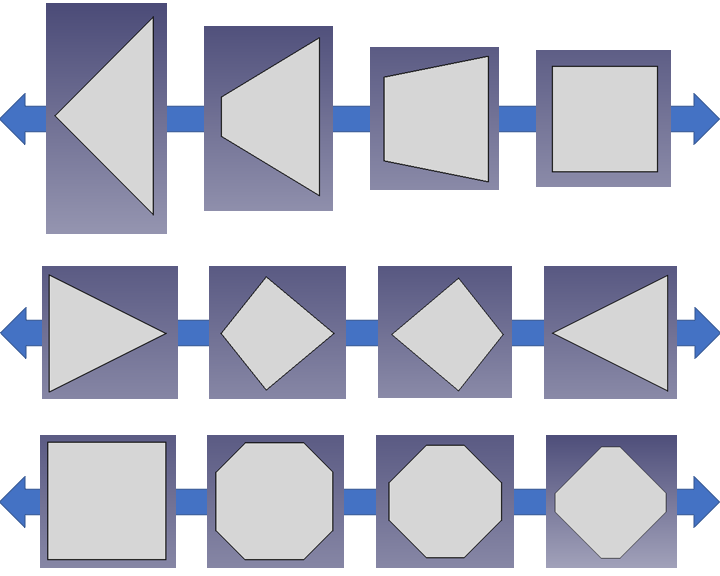
\includegraphics[scale=0.8]{Future_Figs/Cross-Shape-Slide.png}
    \caption{Initial tests of the cross shapes. The left-side of the shape would be the side against the blocker. Two extremes were chosen, with intermediate steps being tested between the two. These are the three sets of extremes used: large triangle to square, triangle with the base against the blocker to triangle with the point against the blocker, and square to truncated diamond.}
    \label{fig:cross-shape-slide}
\end{figure}